% $File: expr.tex
% $Date: Sat Nov 29 16:40:33 2014 +0800
% $Author: jiakai <jia.kai66@gmail.com>

\section{实验设计及实验效果}
关于卷帘快门的参数测量已在\secref{rolling-shutter}中描述,在此不再赘述。

\subsection{基于合成数据的全局运动分析}
% f{{{
使用如下公式合成可控位移的图像,其效果如\figref{synthesis}所示:
\begin{equation}
    f(x, y) = \sin(\omega_x (x + \delta_x)) + \sin(\omega_y y) + 
    \mathcal{N}(0, \sigma^2)
\end{equation}
其中$\delta_x$控制位移,$\sigma$控制噪声,$f(x, y)$被量化到$[0, 255]$间的整数。
\begin{figure}[tb]\begin{center}
    \begin{subfigure}[b]{.35\figwidth}
        \centering
        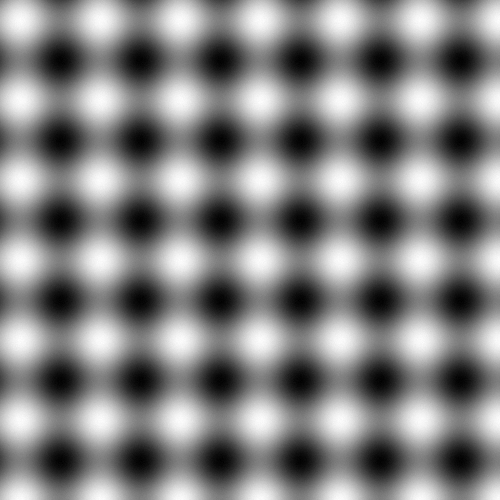
\includegraphics[width=.35\figwidth]{res/synth0.png}
    \end{subfigure}
    \begin{subfigure}[b]{.35\figwidth}
        \centering
        \includegraphics[width=.35\figwidth]{res/synth1.png}
    \end{subfigure}
    \caption{合成数据,$\delta_x = 0.01$pxl, $\sigma = 1.35/255$}
    \label{fig:synthesis}
\end{center}\end{figure}

控制$\delta_x$取不同的值,按上述方法得到的相位差如\figref{synthesis:pd}所示。
\begin{figure}[tb]\begin{center}
    \includegraphics[width=.5\figwidth]{res/synth-pd.png}
    \caption{位移与相位差的关系}
    \label{fig:synthesis:pd}
\end{center}\end{figure}

总的来说,基于合成数据的实验证明了之前想法的可行性,
显示相位差与实际位移线性相关,而且对噪声比较鲁棒,
在$\sigma \le 3/255$时都比较有效,已经远低于一般设备的噪声;
但在$\sigma=0$时出现了较大波动,猜测这是由于量化时取整带来的bias造成的,
而在有噪声时可一定程度上抵消这种bias。而为何在噪声太大时由正相关变成了反相关,
我还没有明确的解释。

% f}}}

\subsection{基于实际数据的全局运动分析与低频信号恢复}
% f{{{

把坐标纸贴在扬声器的震膜上直接拍摄,用扬声器播放10hz, 15hz, 20hz, 25hz的声音,
用Pentax K-01相机拍摄,快门速度为1/2000, iso100, F/5.6, 55mm, 视频为1280x720, 60fps,
H.264编码。

使用上述方法估计全局运动并直接作为采样信号进行FFT,
发现对单频音和多频音均能较好恢复,
多频音的结果如\figref{real:lowfreq}所示。
\begin{figure}[h!]\begin{center}
    \begin{subfigure}[b]{.5\figwidth}
        \includegraphics[width=.5\figwidth]{res/setting.png}
        \caption{实际拍摄情况}
    \end{subfigure}
    \begin{subfigure}[b]{.5\figwidth}
        \includegraphics[width=.5\figwidth]{res/global-recon.png}
        \caption{重建结果,可见对各频率均能较好恢复;
            其中后半部分的振幅偏高是由于拍摄时误碰了实验装置造成整体位移,
            但对结果影响不大}
    \end{subfigure}
    \caption{基于全局运动分析的低频信号重建}
    \label{fig:real:lowfreq}
\end{center}\end{figure}

% f}}}

\subsection{基于实际数据的局部运动分析与高频信号恢复}
% f{{{

这部分尚未完成,仅进行了初步实验。根据之前卷帘快门的模型,
将每行独立看作一帧,对拍摄的两帧图片按各行分别进行运动分析,
并以$18.3\mu s$作为采样间隔。发现对但帧恢复效果仍不稳定。
在大部分情况下频谱能在实际频率附近有尖峰,但有时会出现很混乱情况,
如\figref{real:highfreq}所示。
\begin{figure}[h!]\begin{center}
    \begin{subfigure}[b]{.5\figwidth}
        \includegraphics[width=.5\figwidth]{res/400-0.png}
        \caption{400Hz音频重建情况}
    \end{subfigure}
    \begin{subfigure}[b]{.5\figwidth}
        \includegraphics[width=.5\figwidth]{res/400-1.png}
        \caption{400Hz音频重建混乱的情况}
    \end{subfigure}
    \begin{subfigure}[b]{.5\figwidth}
        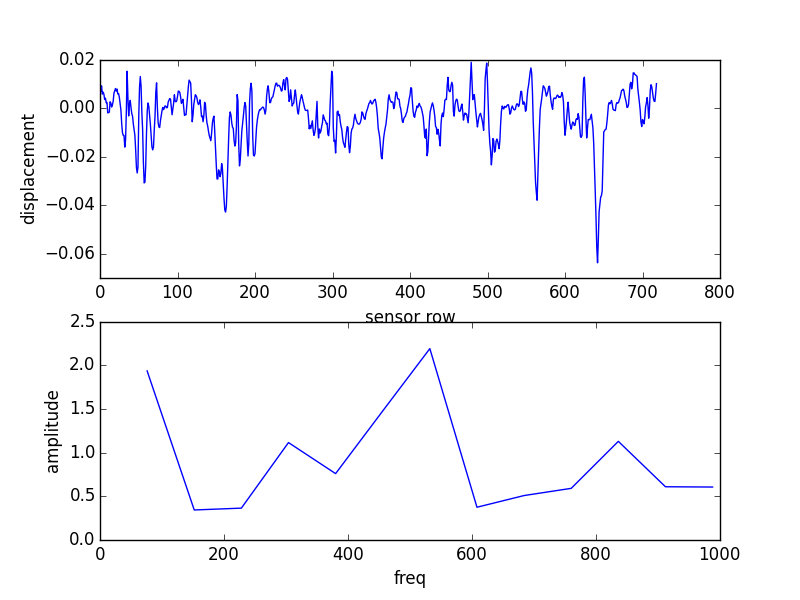
\includegraphics[width=.5\figwidth]{res/500-0.png}
        \caption{500Hz音频重建情况}
    \end{subfigure}
    \begin{subfigure}[b]{.5\figwidth}
        \includegraphics[width=.5\figwidth]{res/500-1.png}
        \caption{500Hz音频重建混乱的情况}
    \end{subfigure}
    \caption{基于局部运动分析的高频信号恢复}
    \label{fig:real:highfreq}
\end{center}\end{figure}

% f}}}

% vim: filetype=tex foldmethod=marker foldmarker=f{{{,f}}} 
